\documentclass[english]{article}
\usepackage[T1]{fontenc}
\usepackage[utf8]{inputenc}
\usepackage{geometry}
\geometry{verbose,tmargin=3.5cm,bmargin=4cm,lmargin=3.8cm,rmargin=3.8cm}

% plots
\usepackage{graphicx}
\graphicspath{ {../plots/} }
\usepackage{calc}
% state diagrams
\usepackage{tikz}
\usetikzlibrary{automata, positioning, arrows}
\tikzset{
  initial text={},
  ->, % makes the edges directed
  node distance=3.5cm, % specifies the minimum distance between two nodes. Change if necessary.
  every state/.style={rectangle, thick, text width=5em, align=center}  % sets the properties for each ’state’ node
}

% newlines instead of indent for paragraphs
\usepackage[parfill]{parskip}
% tables
\usepackage{multirow}

% import natbib and sets bibliography and citation styles
\usepackage[numbers,sort]{natbib}
\bibliographystyle{apalike}

\makeatletter
\usepackage{hyperref}

\makeatother
\usepackage{babel}

% work in progress packages
\newcommand{\citationneeded}{\textsuperscript{\color{blue} [citation needed]}}
\usepackage{easy-todo}

\begin{document}

\listoftodos

\title{Keep your enemies closer and be loud about it}
\author{
  Martin Toman; TUDelft
  \\
  m.toman@student.tudelft.nl
\and
  Dr. Neil Yorke-Smith; TUDelft
  \\
  n.yorke-smith@tudelft.nl
}
\date{25 May 2021}
\maketitle


\begin{abstract}
% The abstract should be short and give the overall idea:
% what is the background, the research questions, what is contribution, and what are the main conclusions.
% It should be readable as a stand-alone text (preferably no references to the paper or outside literature).

\todo{write abstract}
\end{abstract}



\section{Introduction}

% intro - what is prisoner's dilemma
How can we encourage and sustain cooperation? Humans dominate their environments thanks to our ability to cooperate flexibly and at scale, as argued by \citet{harari-sapiens}.
To study the conditions necessary for cooperation to flourish we need a suitable model of an activity with temptations to defect and punishments for doing so.

In 1950, Albert Tucker named a particular two-player exchange game "The Prisoner's Dilemma" \citep{sep-prisoner-dilemma}.
This game elegantly captures the difficulty of the decision between cooperation and defection in a single choice.
Despite being so simple compared to the complexity of the problem it is representing, it was used to model many aspects of behaviour in systems of selfish individuals; and, according to \citet{Axelrod84}, for "discovery of the precise conditions that are necessary and sufficient for cooperation to emerge".

% iterated version + the dilemma
In the case of a one-off exchange, there being no opportunity for a follow-up punishment, the rational behaviour is defection. (This extends to all rounds for a fixed-length game, inductively \citep{Axelrod84}.)
The interesting behaviour arises if there is no end; or, at least, if there is no way for the participants of the game to know when the game ends or even if there is an end.
% reputation importance
An agents has to expect that even a single defection can be infinitely punished by never again being cooperated with \citep{GRIM}.
Such a risk may just not be worth it.

% global reputation system
The defectors can, naturally, only be punished if they can be identified and known to others. This is why services like Ebay or Airbnb have a rating system in place.
Presence of a reputation system has been shown to strongly boost cooperation, as shown by \citet{simple-reputation, public-private-monitoring}.
These studies used groups of volunteers as game participants and explored the effects of various information being public - from only the latest move of the current opponent, to full histories of all moves taken by every participant.

% decentralizing reputation: keeping track internally?
Using human subjects as game participants limited the research to relatively small groups with few rounds; they also used external infrastructure for information passing: eliminating noise, delays, and deliberately wrong information.
As shown by \citet{noise}, not all strategies that perform well in noise-less environments can do so under the presence of noise.

Using external infrastructure for passing information also meant that the transmission speed was uniform for all participants receiving all necessary information in time for their next round of the game.
These are non-trivial idealizations: relaxing them would yield a model closer to real-world systems and could change the results drastically.

In this paper we look at if and how well a local reputation system sustains cooperation and under what conditions does it yield optimal results.
We evaluate the approach under various gossip range and memory length; and comment on the effectiveness of local reputation in enforcing cooperation in spatial prisoner's dilemma.

This was the introduction of the paper, with a short background, motivation, and explanation of the goals of this paper.
In the next section we define the goals explicitly and show the methodology we will use for this research.
Afterwards we show the results with short impartial explanations, followed by discussion of the implications of the results we obtained;
we also connect our results with similar research and comment on the findings.
We close the paper with a short reflection on the ethical aspects and the reproducibility of this paper, after which we summarize and explicitly state our conclusions with some ideas for further research directions.


\section{Methodology}
We aim to measure the effectiveness of local reputation in enforcing cooperation.
To do this we will build a computer simulation of a spatial multi-agent environment.
We will use a Spatial Iterated Prisoner's Dilemma as the principal exchange game for modelling agent interactions.

In this section we define the goals of this paper explicitly,
explain the design of the model and simulations,
and present the measurable properties and evaluation criteria of the model.
We end the section with an explanation of how we will connect our simulation results back to the original question
and what would constitute a confirmation of our hypothesis.

\subsection{Problem Statement}
We will use the prisoner's dilemma game to model agent interactions.
This is a good choice for modelling behaviour of rational and selfish actors.
And will allow us to observe the conditions necessary for cooperation to emerge in the population as well as what makes it sustain itself.

The agents will live in a spatial environment and act independently;
the only mutual interactions will be playing the game with a neighbor and exchanging gossip with nearby agents.
We will vary the range at which the gossip can be exchanges as well as the amount of information which can be included in as single gossip message.
We want to determine the effectiveness of the gossip mechanism in promoting and sustaining cooperation.

\subsection{Simulation Design}
% Typically in general research articles, the second section contains a description of the research methodology, explaining what you, the researcher, is doing to answer the research question(s), and why you have chosen this method.
% This section includes references to necessary background information.

To explore the effects of local reputation, built up via openly gossiping with nearby neighbors,
we will use a computer simulation of a multi-agent spatial environment.
We will base the simulation on the design of \citet{smaldino}.

The model consists of a spatial environment:
square grid with torus (wrapping) bounds,
each cell can be occupied by a single agent.
This is a discreet time model;
at each time step, every agent takes a single turn.
The order in which agents take their turn is randomized in each time step.
Agent's turn is defined by the finite state diagram shown in Figure \ref{fig:agent_behaviour}.
The agents pay a fixed cost to survive ($k = 0.5$) to the next round (agents who deplete their energy die and are removed from the simulation), and try to reproduce once they accumulate enough energy via positive interactions with other agents: PD game wins.

\begin{figure}[h]
  \centering
  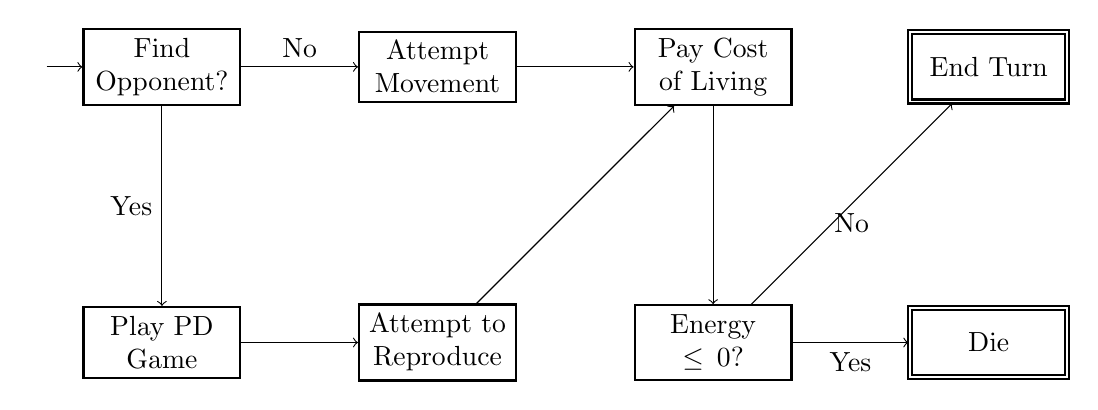
\begin{tikzpicture}

    \node[state, initial] (find_opponent) {Find Opponent?};

    \node[state, below of=find_opponent] (play) {Play PD Game};
    \node[state, right of=play] (reproduce) {Attempt to Reproduce};
    \node[state, right of=find_opponent] (move) {Attempt Movement};
    \node[state, right of=move] (cost) {Pay Cost of Living};
    \node[state, below of=cost] (energy) {Energy $\le 0$?};

    \node[state, accepting, right of=energy] (die) {Die};
    \node[state, accepting, above of=die] (end) {End Turn};

    \draw
      (find_opponent) edge[left] node{Yes} (play)
      (find_opponent) edge[above] node{No}  (move)
      (play) edge[] node{} (reproduce)
      (reproduce) edge[] node{} (cost)
      (move) edge[] node{} (cost)
      (cost) edge[] node{} (energy)
      (energy) edge[below] node{No}  (end)
      (energy) edge[below] node{Yes} (die)
      ;
  \end{tikzpicture}
  \caption{Agent behaviour diagram, derivation of \citationneeded}
  \label{fig:agent_behaviour}
\end{figure}

Every agent can play at most a single PD game in each time step.
Plating a game in the time step is not guaranteed and depends on the spatial configuration of agents, order in which the agents are scheduled, and randomness in choosing an opponent from agent's neighbors.
Similarly, when no opponent is found, movement only happens if an empty cell is found nearby; if there is more than one empty cell, one is chosen randomly.

Agents reproduce by creating a new agent with the same parameters as themselves in an empty neighborhood cell (chosen randomly if more than one, no reproduction if there are no empty cells in the neighborhood).
Reproduction is only attempted if the agent has accumulated at least twice the amount of energy as is the cost of reproduction.
The cost of reproduction is then subtracted from the parent and the offspring is birthed with this energy level.
The cost of reproduction is effectively transferred from the parent to the offspring;
reproducing does not change the net amount of energy in the model.

\begin{table}[h!]
  \centering
  \begin{tabular}{c c||c|c}
    & & \multicolumn{2}{c}{Opponent's move} \\
    & & Cooperate & Defect \\
    \hline\hline

    \multirow{4}{6em}{Player's move}
    & \multirow{2}{5em}{Cooperate}
      & Player:\ \ \ \ \ \ R & Player:\ \ \ \ \ \ S \\
    & & Opponent: R & Opponent: T \\
    \cline{2-4}
    & \multirow{2}{5em}{Defect}
      & Player:\ \ \ \ \ \ T & Player:\ \ \ \ \ \ P \\
    & & Opponent: S & Opponent: P \\
  \end{tabular}

  \caption{Payoff matrix}
  \label{table:payoff}
\end{table}

A single round of the game is defined using a payoff matrix as shown in Table \ref{table:payoff}, with $T > R > P > S$ and $2R > T + S$ \citep{chammah1965}.
Like in the original model \citep{smaldino},
we use $R = 3$ (reward for cooperating),
$T = 5$ (temptation to defect),
$P = 0$ (punishment for mutual defection).
We use a different $S = -1.5$ (sucker's payoff - cooperator got defected) from $S = -1.0$ in the original.

We choose the sucker's payoff value ($S = -1.5$) empirically,
by running simulations of the model and taking note of a value which leads to cooperator extinction relatively quickly.
This choice for the parameter will ensure that, if we reach cooperation, it was caused by the reputation mechanism;
and not because of random interactions in the model.

Environmental harshness of the model is defined by
the sucker's payoff $P$ (social harshness)
and cost to survive $k$ (external harshness).
We will investigate the effect of varying these parameters on our results
and check the effectiveness of gossip across environments of various harshness.

To better suit our needs we will introduce some changes to the original model.
We will reduce the spatial grid size from 100x100, as in the original design, to a more manageable 20x20.
This will allow us to run more simulations with more complex agent behaviour in a manageable time.
We will also decrease the starting number of agents from 1600 to 64: keeping the same percentage of 16\% of the total grid size occupied as in the original model.

This reduction of the environment size (by a factor of 25!) has the effect of significantly increasing the chance of a total extinction of all agents:
caused by the random behaviour of agents exploiting each other until all cooperators are dead and the population of pure defectors cannot sustain itself.
We disregard runs that end in extinction and increase the number of simulation runs to compensate for this.

We will expand the model by giving the agents a (limited size) memory to keep track of past defectors and later to allow them to actively and freely share this knowledge by gossiping with other agents in a given range.
Prior research \citep{memory, reciprocity, adaptive-interaction} has already shown that memory can be an effective tool in promoting cooperation.

Another expansion to the model will be the addition of the localized gossip mechanism.
This will allow agents to consult nearby peers to try and find out the reputation of agents unknown to the agents themselves.
The range at which agents can be contacted and the amount of information which agents provide will be varied.
In the results section, an overview of the effects of varying the parameters of the gossip is shown.
We believe this extension of the model will have a strong positive effect on sustaining cooperation in the model.

The simulation will be implemented in Python using the Mesa\footnote{\url{https://github.com/projectmesa/mesa}} framework.

\subsection{Simulation Evaluation}

To determine the effectives of gossip in promoting cooperation, we will observe the rate of convergence to a population of cooperators, stopping the simulation once stable equilibrium is achieved.
To verify that this is indeed an equilibrium by letting the simulation run longer and checking that the general behaviour does not change.
We will also observe the maximal population size of defectors which can sustain itself alongside the cooperators.

The main properties measured about the model will be the saturation of cooperator and defector populations.
We will measure the saturation as the fraction of agents of the type alive in the model divided by
the total carrying capacity of the population: 50\% of all the cells.
This differs from the measure of agent type frequency used by \citet{smaldino};
we have chosen to use the saturation measurement because with the decreased size model we encounter total extinction more often,
and with the gossip extension aim to speed up defector extinction.

We believe the measure of agent type saturation is clearer and easier to understand
as the relative population sizes do not influence the measure of the other type (as frequency does).
Consider the case of 10 defector and 10 cooperator with maximal carrying capacity of 20 for either type:
saturation is 50\% for both agent types, and cooperator frequency is also 50\%.
Now 10 more cooperators are born:
defector saturation stays at 50\%, cooperator saturation increases to 100\%,
and the cooperator frequency changes to 33.3\%.
Using the saturations explain what happened more clearly at the cost of having to present 2 complementary charts for each measurement:
one for cooperator and one for defector saturation.

Measuring both, the cooperator and the defector saturation might seem redundant at first.
However, the relationship between them is highly nonlinear and depends on many factors
as will be shown in the results section.

We will also record characteristic patterns formed by the populations as influenced by different parameters.
We do this, because it was shown by earlier work \citep{spatial-patterns} that in Spatial Prisoner's Dilemma interesting patterns can emerge over time.
These patterns are very similar to patterns occurring in nature, which are often created by reaction-diffusion processes.
This suggests a deeper link between our model and natural processes.



\section{Results}
Now we present the results of our simulation
with commentary on the setup and meaning of the results.
We show the results impartially and let the data do most of the talking.
A thorough explanation of the data in the context of similar research
with explanation of wider implications will be in the next section.

We start by presenting the behaviour of the plain (baseline) model in the first subsection,
then we expand it by adding memory and show how this alters the results obtained,
afterwards we enable communication (gossip) between agents and rerun the simulations once again.

After making the comparisons between the behaviour as influenced by various extensions we look a closer look at the robustness of the gossip model against environmental harshness: both social (sucker's payoff $S$) and external (cost of living $k$).

We wrap this section by comparing the characteristic spatial patterns of the models.


\subsection{Baseline model}
First we look at the plain model with 0-memory and no communication (gossip) between agents.
This is a replication of \citet{smaldino}; with some alterations.
As explained in the model design subsection, we modify the original model slightly.
We decrease the size of the grid from 100x100 to 20x20,
and decrease the starting agent count from 1600 to 64.
We will keep torus (wrapping) bounds, as in the original paper.
We will also keep some other parameters:
starting energy will be randomly chosen for each agent to be between 1 and 49 (inclusive),
energy cost to reproduce is 50 (agent has to accumulate at least 100 energy and reproduces by transferring 50 to the offspring),
and the maximum energy an agent can hold is 150.

For the PD game payoffs we will use $R = 3$, $T = 5$, $S = -1.5$, and $P = 0$.
And the living cost $k = 0.5$.
These values were shown to lead to the cooperators struggling to survive
and maintain their numbers \citep{smaldino}.

Unless otherwise noted, we will use these parameters for all simulation runs.

We begin by exploring the robustness of the model against social harshness - represented by the $S$ (sucker's payoff) parameter.
In Figure \ref{fig:agent_sat/S-memory0gossip0} we present the results of running the simulation for $2.5 \leq S \leq 0.0$.
We observe that $S = -1.5$ leads to total extinction in the model by step 500;
we will use this value for the parameter for further simulations to determine the effectiveness of memory and the gossip mechanism in promoting and sustaining cooperation.

\begin{figure}[!h]
  \centering
  \makebox[\textwidth]{
    \includegraphics[width=\paperwidth-4cm]{saturation&S-memory0+gossip0_100steps_large}
  }
  \makebox[\textwidth]{
    \includegraphics[width=\paperwidth-4cm]{saturation&S-memory0+gossip0_250steps_large}
  }
  \makebox[\textwidth]{
    \includegraphics[width=\paperwidth-4cm]{saturation&S-memory0+gossip0_500steps_large}
  }
  \makebox[\textwidth]{
    \includegraphics[width=\paperwidth-4cm]{saturation&S-memory0+gossip0_1000steps_large}
  }
  \caption{Agent type saturation for various $S$ (sucker's payoff) after 100, 250, 500, 1000 steps; SD of 30 simulation runs, outliers removed}
  \label{fig:agent_sat/S-memory0gossip0}
\end{figure}


\subsection{Remember defectors}
We have determined the value of for the parameter $S = -1.5$ which repeatably leads to extinction of the whole population by step 500.

Now we expand the model by allowing agents to remember some fixed number of most recent defectors encountered. We will examine how varying the number of defectors which can be remembered (memory size) influences the cooperator and defector saturations.

\begin{figure}[]
  \centering
  \makebox[\textwidth]{
    \includegraphics[width=\paperwidth-4cm]{saturation&memory_size-gossip0_100steps_large}
  }
  \makebox[\textwidth]{
    \includegraphics[width=\paperwidth-4cm]{saturation&memory_size-gossip0_150steps_large}
  }
  \makebox[\textwidth]{
    \includegraphics[width=\paperwidth-4cm]{saturation&memory_size-gossip0_175steps_large}
  }
  \makebox[\textwidth]{
    \includegraphics[width=\paperwidth-4cm]{saturation&memory_size-gossip0_500steps_large}
  }
  \caption{Agent type saturation for various memory sizes after 100, 150, 175, 500 steps; SD of 30 simulation runs, outliers removed}
  \label{fig:agent_sat/memory_size}
\end{figure}

The effect of various memory sizes on the agent type saturations are shown in Figure \ref{fig:agent_sat/memory_size}.
\todo{conclusion on memory effect : both live well, cooperators have an edge and are faster to saturate}


\subsection{Gossip about defectors}
\todo{gossip model: defectors die off quickly}

\todo{check robustness against harshness}


\subsection{Spatial patterns}
\todo{characteristic patterns}



\section{Discussion}
% Results can be compared to known results and placed in a broader context.
% Provide a reflection on what has been concluded and how this was done.
% Then give a further possible explanation of results.

% You may give this section another name, or merge it with the one before or the one hereafter.
\todo{write discussion: compare with the human reputation experiment}



\section{Responsible Research}
We recognize the inherent difficulties in conducting ethical and sustainable research.
We take the following actions to ensure this paper is ethically good
and can be reproduced by others, to provide a solid foundation for others to reproduce, reuse, and build upon this paper.

% Reflect on the ethical aspects of your research and discuss the reproducibility of your methods.
\subsection{Ethical aspects}
This paper focused on exploring the effects of reputation on promoting and sustaining cooperation.
We believe this research is ethically good and our conscience is clean about the methods used and conclusions reach, as well as all other aspects of this paper.

While we cannot ensure the findings of this paper will not be misused by others. We implore all reader's to always strive for the highest ethical ideals.
Let's all be excellent.

\subsection{Reproducibility}
We want to make this paper a good foundation for future work and as such we provide all source materials for this paper: including the code files for running the simulations and evaluating results, the \LaTeX\ files for this paper, and anything else used while conducting this research.

Next, we use Nix Flake\footnote{\url{https://nixos.wiki/wiki/Flakes}} to capture the exact versions of all software, libraries, and packages used for this research \citep{nix}. All of this is captured together in and provided as a fully reproducible environment.
We hope that by doing this it becomes easy to reproduce our results and provide a good foundation environment for other researchers to quickly kick-start their research.

Our model itself is implemented in a Jupyter Notebook\footnote{\url{https://jupyter.org/}} and care was taken to keep the total amount of dependencies as low as possible and to stick to the most standard dependencies whenever possible.
We hope others will appreciate this by building upon our research and uncovering wonderful conclusions.



\section{Conclusions and Future Work}
% ideally, this section can stand on its own: it should be readable without having read the earlier sections.
\todo{summary intro}

\subsection{Our conclusions}
% Summarize the research question(s) and the answers to the research question(s).
% Make statements.
% Highlight interesting elements.
\todo{conclude}

\subsection{Future work}
% Discuss open issues, possible improvements, and new questions that arise from this work; formulate recommendations for further research.
\todo{outline future work: noise, more complex agents, probabilistic strategies}



\pagebreak
\bibliography{references}

\end{document}
